\usepackage{../SoftVarE-SlideTemplate/beamerthemeuulm} % use the inofficial uulm beamer theme
\uulmlogos{,uulm,,unibe,,ovgu-blue,}
\setmycolumnsdefault{animation=keep} % animate all columns per default

\title{Software Product Lines} % short title is used for the slide footer but optional

% TODO if we give each lecture a specific number this could be used as default value here, simplifying the highlighting at beginning and end of each lecture (could be done in header and footer essentially)
\newcommand{\emphifequal}[2]{\ifthenelse{\equal{#1}{#2}}{\color{blue}\bfseries}{}}
\newcommand{\lectureseriesoverview}[1][]{ % shown at the start and end of each part
	\begin{mycolumns}[columns=3,t,animation=none]
		\mydefinition{\emphifequal{#1}{I}Part I: Ad-Hoc Approaches for Variability}{
			\begin{enumerate}
				\item {\emphifequal{#1}{1}Introduction}
				\item {\emphifequal{#1}{2}Runtime Variability and Design Patterns}
				\item {\emphifequal{#1}{3}Compile-Time Variability with Clone-and-Own}
			\end{enumerate}
		}
	\mynextcolumn
		\mydefinition{\emphifequal{#1}{II}Part II: Modeling and Implementing Features}{
			\begin{enumerate}
				\setcounter{enumi}{3}
				\item {\emphifequal{#1}{4}Feature Modeling}
				\item {\emphifequal{#1}{5}Conditional Compilation}
				\item {\emphifequal{#1}{6}Modular Features}
				\item {\emphifequal{#1}{7}Languages for Features}
				\item {\emphifequal{#1}{8}Development Process}
			\end{enumerate}
		}
	\mynextcolumn
		\mydefinition{\emphifequal{#1}{III}Part III: Quality Assurance and Outlook}{
			\begin{enumerate}
				\setcounter{enumi}{8}
				\item {\emphifequal{#1}{9}Feature Interactions}
				\item {\emphifequal{#1}{10}Product-Line Analyses}
				\unlessuniversity{wernigerode}{
					\item {\emphifequal{#1}{11}Product-Line Testing}
				}
				\ifuniversity{ulm}{
					\item {\emphifequal{#1}{13}Current Research Topics}
				}
				\unlessuniversity{wernigerode}{
					\item {\emphifequal{#1}{12}Evolution and Maintenance}
				}
				\ifuniversity{wernigerode}{
					\item {\emphifequal{#1}{11}Cost Estimation}
				}
			\end{enumerate}
		}
	\end{mycolumns}
}

% emphasizing links
\hypersetup{linkcolor = black, citecolor = black, filecolor = black, runcolor = black, urlcolor = red, colorlinks=true}

% GRAPHICSPATH

\makeatletter
\newcommand{\setpaths}[1]{
	\graphicspath{#1} % for loading pictures
	\def\input@path{#1} % for loading picture sources
}
\makeatother

% load href target from file: \href{file.txt}{text}
\newcommand\hreffile[1]{%
	\CatchFileDef\myurl{#1}{\catcode`\#=12\catcode`\%=12\endlinechar=-1}%
	\expandafter\href\expandafter{\myurl}}
\newcommand{\pic}[2][]{%
	\IfFileExists{#2.txt}{\hreffile{#2.txt}}{}{\includegraphics[#1]{#2}}}

\setpaths{
	{../SoftVarE-SlideTemplate/pics/logos/}
	{../SoftVarE-SlideTemplate/pics/nature/}
	{../SoftVarE-SlideTemplate/pics/uulm/}
	{../SoftVarE-Papers/}
	{../SoftVarE-Slides/}
	{../pics/}
	{../pics/aop/}
	{../pics/bikes/}
	{../pics/buildsystems/}
	{../pics/cars/}
	{../pics/cloneandown/}
	{../pics/components/}
	{../pics/configurators/}
	{../pics/elevators/}
	{../pics/fop/}
	{../pics/frameworks/}
	{../pics/graphs/}
	{../pics/interactions/}
	{../pics/linux/}
	{../pics/literature/}
	{../pics/lego/}
	{../pics/logos/}
	{../pics/magdeburg/}
	{../pics/mindmaps/}
	{../pics/people/}
	{../pics/preprocessors/}
	{../pics/products/}
	{../pics/projectcartoon/}
	{../pics/runtimevariability/}
	{../pics/services/}
	{../pics/testing/}
	{../pics/variabilitymodels/}
	{../pics/versioncontrol/}
	{../pics/wernigerode/}
	{../pics/xkcd/}
	{../EagleoutIce-fancyqr/}
}

% IMPORTED PACKAGES

\usepackage{multicol} % used temporarily for the lecture overview
\usepackage{stmaryrd} % \lightning in modeling lecture
\usepackage{catchfile} % read picture sources from files
\usepackage{silence} % ignore some warnings
\WarningFilter{latex}{You have requested package} % ignore warning for loading packages from submodules
\usepackage{fancyqr} % QR codes for practice task, credits to Florian Sihler
\usepackage{ifthen} % \ifuniversity
\usepackage[absolute,overlay]{textpos} % absolute positioning in myframeicon with textblock*

% INCLUDED TEMPLATE FILES

% default colors
% used in standalone pictures and when no university is selected
\definecolor{black}{HTML}{000000}
\definecolor{green}{HTML}{33BB33}
\definecolor{red}{HTML}{BB3333}
\definecolor{orange}{HTML}{BB6600}
\definecolor{blue}{HTML}{3333BB}
\definecolor{uulmaccent}{HTML}{999999}

\definecolor{uulmlogoblue}{named}{blue}
\definecolor{uulmblue}{named}{blue}

\ifdarkmode
	\colorlet{green}{green!85!white}
	\colorlet{red}{red!85!white}
	\colorlet{orange}{orange!85!white}
	\colorlet{blue}{blue!85!white}
	\setbeamercolor{section in toc shaded}{fg=black}
	\setbeamertemplate{section in toc shaded}[default][50]
\fi

% TYPICAL COMMANDS FOR LECTURES

\renewcommand{\emph}[1]{{\color{blue}\textbf{#1}}}

\newcommand{\deutsch}[1]{{\color{blue}(#1)}}
\newcommand{\deutschertitel}[1]{{\tiny\deutsch{#1}}}

\newcommand{\mycite}[1]{``#1''}
\newcommand{\mycitebegin}{``}
\newcommand{\myciteend}{''}
\newcommand{\mytitlesource}[1]{{\tiny\normalfont\mbox{[#1]}}}
\newcommand{\mysource}[1]{\ifthenelse{\equal{#1}{}}{}{\phantom{.}~\hfill~\mytitlesource{#1}}}
\newcommand{\mypage}[1]{, p.~#1}
\newcommand{\mypages}[1]{, pp.~#1}

\newcommand{\todo}[1]{{\color{red}\textbf{[#1]}}}
\newcommand{\fodo}[1]{\todo{\footnote{\todo{#1}}}}
\newcommand{\todots}{\todo{\ldots}}

\newcommand{\textheightwithtitle}{.825\textheight}
\newcommand{\textheightwithouttitle}{.975\textheight}

\newcommand{\lessonslearned}[3]{
	\subsection{Summary}
	\begin{frame}{\insertsection{} -- \insertsubsection}
		\leftandright{
			\mydefinition{Lessons Learned}{
				\begin{itemize}
					#1
				\end{itemize}
			}
			\uncover<2->{\mynote{Further Reading}{
				\small % references take space, can be a little smaller
				\begin{itemize}
					#2
				\end{itemize}
			}}
		}{
			\uncover<3->{\myexample{Practice}{
				\begin{itemize}
					#3
				\end{itemize}
			}}
		}
	\end{frame}
}

% COMMANDS FOR PROPOSITIONAL FORMULAS AND MATHEMATICAL NOTATIONS

\newcommand{\sem}[1]{\ensuremath{\llbracket #1 \rrbracket}} % semantics brackets
\newcommand{\pand}{\wedge} % conjunction
\newcommand{\por}{\vee} % disjunction
\newcommand{\pnot}{\neg} % negation
\newcommand{\pequals}{\leftrightarrow} % biconditional
\newcommand{\npequals}{\nleftrightarrow} % exclusive disjunction
\newcommand{\mequals}{\Leftrightarrow} % equivalence (meta-level)
\newcommand{\pimplies}{\rightarrow} % conditional
\newcommand{\mimplies}{\Rightarrow} % implication (meta-level)
\newcommand{\defeq}{\vcentcolon=} % defining equals
\newcommand{\power}[1]{\mathcal{P}(#1)} % power set
\newcommand{\refslide}[1]{\hyperlink{#1}{(see Slide \autoref{#1})}} % link to slide
\newcommand{\fs}[1]{\ensuremath{{\color{green}#1}}} % selected feature
\newcommand{\fd}[1]{\ensuremath{{\color{red}#1}}} % deselected feature
\newcommand{\cfg}[3][0]{\ensuremath({{\only<#1>{\color{green}}\{#2\}}, {\only<#1>{\color{red}}\{#3\}})}} % configuration

\usepackage{mathtools} % required for absolute value in modeling lecture
\DeclarePairedDelimiter\abs{\lvert}{\rvert} % absolute value

% COMMANDS TO INCLUDE XKCDs

\newcommand{\xkcd}[2]{
	\href{https://xkcd.com/#1/}{\includegraphics[#2]{#1}}
}
\newcommand{\xkcdframe}[1]{
	\begin{frame}
		\centering%
		\xkcd{#1}{height=80mm}
	\end{frame}
}
\newcommand{\widexkcdframe}[1]{
	\begin{frame}
		\xkcd{#1}{width=\linewidth}
	\end{frame}
}

% COMMANDS TO SIMPLIFY USAGE OF THE PROJECT CARTOON

\newcommand{\projectcartoonwidth}{.19} % default value for 5 tiles
\newcommand{\projectcartoon}[2]{\projectcartoonimage{sepia/cell_#1}{#2}}
\newcommand{\hprojectcartoon}[2]{\projectcartoonimage{alpha/cell_#1}{#2}}
\newcommand{\projectcartoonimage}[2]{
	\begin{minipage}[t]{\projectcartoonwidth\linewidth}
		\centering
		\href{http://web.archive.org/web/20191029221320/http://www.projectcartoon.com/}{\includegraphics[width=\linewidth]{#1}}\\#2
	\end{minipage}\hfill
}
\newcommand{\waterfallcartoon}{
	\hprojectcartoon{02}{Analysis}%
	\hprojectcartoon{03}{Design}%
	\hprojectcartoon{04}{Implementation}%
	\hprojectcartoon{05}{Testing}%
	\hprojectcartoon{10}{Maintenance}%
}
%\uncover<1->{\hprojectcartoon{01}{how the customer explained it}} % requirements
%\uncover<1->{\hprojectcartoon{02}{how the project leader understood it}} % modeling
%\uncover<1->{\hprojectcartoon{03}{how the analyst designed it}} % architecture and design
%\uncover<1->{\hprojectcartoon{04}{how the programmer implemented it}} % implementation
%\uncover<1->{\hprojectcartoon{05}{what the beta testers received}} % testing
%\uncover<1->{\hprojectcartoon{06}{how the business consultant described it}} % process
%\uncover<1->{\hprojectcartoon{07}{how the project was documented}} % documentation?
%\uncover<1->{\hprojectcartoon{08}{what operations installed}} % devops/continuous integration?
%\uncover<1->{\hprojectcartoon{09}{how the customer was billed}} % management (pricing)
%\uncover<1->{\hprojectcartoon{10}{how it was supported}} % maintenance
%\uncover<1->{\hprojectcartoon{11}{what marketing advertised}} % product lines. marketing? reuse?
%\uncover<1->{\hprojectcartoon{12}{when it was delivered}} % configuration management. continous delivery?
%\uncover<1->{\hprojectcartoon{13}{what the customer really needed}} % customer / SE II
%\uncover<1->{\hprojectcartoon{14}{what the digg effect can do to your site}} % ???
%\uncover<1->{\hprojectcartoon{15}{the disaster recover plan}} % ???
%\uncover<1->{\hprojectcartoon{16}{the open source version}} % open source (licensing)
%\uncover<1->{\hprojectcartoon{17}{how it performed under load}} % compilation and static analyses. quality assurance? performance?
%\uncover<1->{\hprojectcartoon{18}{how patches were applied}} % evolution

\usepackage{xstring}

\newcommand{\featureDiagramConfigurableDatabase}[1][]{
	\featureDiagram{
		\subnode{ConfigDB#1}{ConfigDB},concrete
		[\subnode{API#1}{API},abstract,mandatory
			[\subnode{Get#1}{Get},concrete,or]
			[\subnode{Put#1}{Put},concrete]
			[\subnode{Delete#1}{Delete},concrete]
		]
		[\subnode{Transactions#1}{Transactions},concrete,optional]
		[\subnode{OS#1}{OS},abstract,mandatory
			[\subnode{Windows#1}{Windows},concrete,alternative]
			[\subnode{Linux#1}{Linux},concrete]
		]
	}

	$Transactions \pimplies Put \por Delete$
}

\newcommand{\featureDiagramWaffle}{
	\featureDiagram{
		Waffle,concrete
		[Topping,optional,abstract
			[Sugar,concrete,or]
			[Cream,concrete]
			[Cherries,concrete]
			[Nutella,concrete]
			[Crumbles,concrete
				[Chocolate,concrete,alternative]
				[Colored,concrete]]]
		[Accessories,abstract,mandatory
			[Plate,concrete,mandatory]
			[Fork,concrete,optional
				[Plastic,concrete,alternative]
				[Wood,concrete]]]
		[Customer,abstract,mandatory
			[Adult,abstract,alternative]
			[Child,abstract]]
	}

	$Sugar$\\
	$Cherries \pimplies Sugar \pand Fork$\\
	$Nutella \por Crumbles \pimplies Child$\\
	$Fork \pimplies Adult$
}

\newcommand{\featureDiagramGraphs}{
	\featureDiagram{
		Graph,concrete
		[Nodes,mandatory,abstract
			[Colored,optional,concrete]]
		[Edges,mandatory,abstract
			[Directed,optional,concrete]
			[Weighted,optional,concrete]]
		[Algorithms,mandatory,abstract,
			[ShortestPath,optional,concrete]]
	}

	$ShortestPath \pimplies Weighted$
}

\newcommand{\featureDiagramEightOptionalFeatures}{
	\featureDiagram{
		SPL,abstract
		[F1,concrete,optional]
		[F2,concrete,optional]
		[F3,concrete,optional]
		[F4,concrete,optional]
		[F5,concrete,optional]
		[F6,concrete,optional]
		[F7,concrete,optional]
		[F8,concrete,optional]
	}
}

\newcommand{\featureDiagramLego}{
	\featureDiagram{
		Lego Manikin,abstract
			[Headpiece,abstract,optional
				[Helmet,concrete,alternative]
				[Hat,concrete]]
			[Head,concrete,mandatory]
			[Item,abstract,optional
				[Brush,concrete,or]
				[Phone,concrete]]
			[Shirt,concrete,mandatory]
			[Pants,abstract,mandatory
				[Red,concrete,alternative]
				[Blue,concrete]]
	}
	%\\$Helmet \pimplies \pnot Phone$
}


% STYLE COMMANDS FOR FEATURE DIAGRAMS

\usepackage{forest}
\usepackage{xcolor}
\usetikzlibrary{angles}
\usetikzlibrary{tikzmark}
\definecolor{drawColor}{RGB}{128 128 128}
\newcommand{\circleSize}{0.175em}
\newcommand{\angleSize}{0.75em}

\forestset{
	/tikz/mandatory/.style={
		circle,fill=drawColor,
		draw=drawColor,
		inner sep=\circleSize
	},
	/tikz/optional/.style={
		circle,
		fill=white,
		draw=drawColor,
		inner sep=\circleSize
	},
	featureDiagram/.style={
		for tree={
			text depth = 0,
			parent anchor = south,
			child anchor = north,
			draw = drawColor,
			edge = {draw=drawColor},
		}
	},
	featureDiagramEmpty/.style={
	},
	/tikz/abstract/.style={
		fill = blue!85!cyan!5,
		draw = drawColor
	},
	/tikz/concrete/.style={
		fill = blue!85!cyan!20,
		draw = drawColor
	},
	mandatory/.style={
		edge label={node [mandatory] {} }
	},
	optional/.style={
		edge label={node [optional] {} }
	},
	or/.style={
		tikz+={
			\path (.parent) coordinate (A) -- (!u.children) coordinate (B) -- (!ul.parent) coordinate (C) pic[fill=drawColor, angle radius=\angleSize]{angle};
		}	
	},
	/tikz/or/.style={
	},
	alternative/.style={
		tikz+={
			\path (.parent) coordinate (A) -- (!u.children) coordinate (B) -- (!ul.parent) coordinate (C) pic[draw=drawColor, angle radius=\angleSize]{angle};
		}	
	},
	/tikz/alternative/.style={
	},
	/tikz/placeholder/.style={
	},
	collapsed/.style={
		rounded corners,
		no edge,
		for tree={
			fill opacity=0,
			draw opacity=0,
			l = 0em,
		}
	},
	/tikz/hiddenNodes/.style={
		midway,
		rounded corners,
		draw=drawColor,
		fill=white,
		minimum size = 1.2em,
		minimum width = 0.8em,
		scale=0.9
	},
}

\newcommand{\legend}{
	\matrix [draw=drawColor,anchor=north west] at (current bounding box.north east) {
		\node [label=center:\underline{Legend:}] {}; \\
		\node [abstract,label=right:Abstract Feature] {}; \\
		\node [concrete,label=right:Concrete Feature] {}; \\
		\node [mandatory,label=right:Mandatory] {}; \\
		\node [optional,label=right:Optional] {}; \\
			\filldraw[drawColor] (0.1,0) - +(-0,-0.2) - +(0.2,-0.2)- +(0.1,0);
			\draw[drawColor] (0.1,0) -- +(-0.2, -0.4);
			\draw[drawColor] (0.1,0) -- +(0.2,-0.4);
			\fill[drawColor] (0,-0.2) arc (240:300:0.2);
		\node [or,label=right:Or Group] {}; \\
		\draw[drawColor] (0.1,0) -- +(-0.2, -0.4);
			\draw[drawColor] (0.1,0) -- +(0.2,-0.4);
			\draw[drawColor] (0,-0.2) arc (240:300:0.2);
		\node [alternative,label=right:Alternative Group] {}; \\
	};
}

\newcommand{\featureDiagramWithLegend}[1]{
	\begin{forest}
		featureDiagram[#1]
		\matrix [anchor=north west] at (current bounding box.north east) {
			\node [placeholder] {}; \\
		};
		{\small\legend}
	\end{forest}
}

\newcommand{\featureDiagram}[1]{
	\begin{forest}
		featureDiagram[#1]
	\end{forest}
}

\newcommand{\featureDiagramLegend}{
	\begin{forest}
		featureDiagramEmpty[]
		{\small\legend}
	\end{forest}
}

\newcommand{\featureDiagramOverlay}[1]{
	\begin{tikzpicture}[overlay,remember picture]
		#1
	\end{tikzpicture}
}

\newcommand{\featureEmph}[2][draw=black]{
		\foreach \f in {#2} {
			\node [fit=\f,fill opacity=0.4,line width=0.6pt,rounded corners,#1] {};
		}
}

\newcommand{\featureDeemph}[2][fill=white]{
	\foreach \f in {#2} {
		\node [fit=\f,fill opacity=0.4,line width=0.6pt,rounded corners,#1] {};
	}
}

\newcommand{\featureSelected}[1]{
	\featureEmph[fill=green,draw=green,fill opacity=0.1,draw opacity=0.2]{#1}
}

\newcommand{\featureDeselected}[1]{
	\featureEmph[fill=red,draw=red,fill opacity=0.1,draw opacity=0.2]{#1}
}

 % TODO merge into template?
\usepackage{listings}
\usepackage[normalem]{ulem}
\tcbuselibrary{listings}

\newcommand{\definelanguage}[2]{
	\lstdefinelanguage{#1}{#2}
	\lstnewenvironment{#1}[1][]{\lstset{language=#1,##1}}{}
	\newtcblisting{#1tight}[2][]{fancy@tightboxstyle={top=-6pt,bottom=-6pt}{##2}{fancy@box@example}{example},listing only,listing options={language=#1,##1}}
}

% listing style inherited by all languages
\lstset{
	numbers=none, % where to put the line-numbers
	showspaces=false, % show spaces with underscores
	showstringspaces=false, % underline spaces within strings
	showtabs=false, % show tabs within strings with underscores
	tabsize=2, % sets default tabsize to 2 spaces
	breaklines=true, % sets automatic line breaking
	breakatwhitespace=false,
	columns=fullflexible,
	commentstyle=\color{black!50}
}

% easy font size selection
\lstdefinestyle{small}{basicstyle=\sf\small\selectfont}
\lstdefinestyle{footnotesize}{basicstyle=\sf\footnotesize\selectfont}
\lstdefinestyle{scriptsize}{basicstyle=\sf\scriptsize\selectfont}
\lstdefinestyle{tiny}{basicstyle=\sf\tiny\selectfont}

% language-specific styles
\definelanguage{code}{
	style=small,
	language=Java,
	keywordstyle=\bf,
	moredelim=**[is][\color{lecturegreen}]{@}{@},
	moredelim=**[is][\color{lecturered}]{?}{?},
	moredelim=**[is][\color{lectureblue}]{~}{~},
	moredelim=[is][\sout]{|}{|},
}

\definelanguage{uvl}{
	alsoletter={=, >, |},
	morekeywords={features, constraints, namespace, mandatory, optional, or, alternative, abstract, =>, |}
}

\definelanguage{dimacs}{
	alsoletter={0},
	morekeywords={p, cnf, 0},
	morecomment=[f]{c},
}

\definelanguage{kconfig}{
	keepspaces=true,
	morekeywords={config, bool, default, if, help, def_bool, depends, on, select},
	morecomment=[l]{\#},
	morestring=*[d]{"},
	literate={-}{{-}}1,
}

\definelanguage{kbuild}{
	morekeywords={config, bool, default, if, help, def_bool, depends, on, select},
	morecomment=[l]{\#},
	moredelim=**[is][\color{lecturered}]{~}{~},
	moredelim=**[is][\color{lecturegreen}]{?}{?},
	literate={-}{{-}}1,
}

\definelanguage{cpp}{
	language=C++,
	morekeywords={elifdef,elifndef},
	moredelim=**[is][\color{lecturegreen}\bfseries\itshape]{~}{~},
	moredelim=**[is][\color{lecturered}\bfseries\itshape]{@}{@}
} % TODO merge into template?

% LINKED LITERATURE

\newcommand{\alhajjajiprioritization}{\href{https://dx.doi.org/10.1007/s10270-016-0569-2}{Al-Hajjaji~et~al.~2019}}
\newcommand{\analysisstrategies}{\href{https://raw.githubusercontent.com/SoftVarE-Group/Papers/main/2014/2014-CSUR-Thuem.pdf}{Thüm~et~al.~2014}}
\newcommand{\backgroundcolors}{\href{https://link.springer.com/article/10.1007/s10664-012-9208-x}{Feigenspan~et~al.~2013}}
\newcommand{\bakarnaturallanguage}{\href{https://doi.org/10.1016/j.jss.2015.05.006}{Bakar~et~al.~2015}}
\newcommand{\batorygrammars}{\href{https://link.springer.com/chapter/10.1007/11554844_3}{Batory~2005}}
\newcommand{\czarneckithereandbackagain}{\href{https://ieeexplore.ieee.org/document/4339252}{Czarnecki~and~Wasowski~2007}}
\newcommand{\cide}{\href{https://wwwiti.cs.uni-magdeburg.de/iti_db/forschung/cide/}{CIDE}}
\newcommand{\dimacsformat}{\href{https://beyondnp.org/static/media/uploads/docs/satformat.pdf}{DIMACS~1993}}
\newcommand{\evaluatingsharpsatsolverslink}[1]{\href{https://raw.githubusercontent.com/SoftVarE-Group/Papers/main/2020/2020-VaMoS-Sundermann.pdf}{#1}}
\newcommand{\evaluatingsharpsatsolvers}{\evaluatingsharpsatsolverslink{Sundermann~et~al.~2020}}
\newcommand{\essentialconfigurationcomplexitylink}[1]{\href{https://raw.githubusercontent.com/SoftVarE-Group/Papers/main/2016/2016-ASE-Meinicke.pdf}{#1}}
\newcommand{\essentialconfigurationcomplexity}{\essentialconfigurationcomplexitylink{Meinicke~et~al.~2016}}
\newcommand{\featureide}{\href{https://link.springer.com/book/10.1007\%2F978-3-319-61443-4}{Meinicke~et~al.~2013}}
\newcommand{\featurecommander}{\href{https://www.tu-chemnitz.de/informatik/ST/research/material/xenomai/}{Feature~Commander}}
\newcommand{\fortyproductlines}{\href{https://dl.acm.org/doi/abs/10.1145/1806799.1806819}{Liebig~et~al.~2010}}
\newcommand{\fospl}{\href{https://link.springer.com/book/10.1007/978-3-642-37521-7}{Apel~et~al.~2013}}
\newcommand{\foda}{\href{https://resources.sei.cmu.edu/library/asset-view.cfm?assetid=11231}{Kang~et~al.~1990}}
\newcommand{\gof}{\href{https://learning.oreilly.com/library/view/design-patterns-elements/0201633612/}{Gang of Four}}
\newcommand{\hentzesolutionspacesampling}{\href{https://dl.acm.org/doi/abs/10.1145/3564719.3568695}{Hentze~et~al.~2022}}
\newcommand{\icpl}{\href{https://dl.acm.org/doi/10.1145/2362536.2362547}{Johansen~et~al.~2012}}
\newcommand{\krieterpresenceconditioncoverage}{\href{https://arxiv.org/abs/2205.15180}{Krieter~et~al.~2022}}
\newcommand{\lehmanslaws}{\href{https://ieeexplore.ieee.org/iel3/5031/13795/00637156.pdf}{Lehman et al.\ 1997}}
\newcommand{\ludewiglichter}{\href{https://learning.oreilly.com/library/view/-/9781457184932/?ar}{Ludewig and Lichter}}
\newcommand{\oosoftwareconstruction}{\href{https://dl.acm.org/doi/10.5555/261119}{Meyer~1997}}
\newcommand{\reducingconfigurations}{\href{https://doi.org/10.1145/1960275.1960284}{Kim~et~al.~2011}}
\newcommand{\samplingsurvey}{\href{https://raw.githubusercontent.com/SoftVarE-Group/Papers/main/2018/2018-SPLC-Varshosaz.pdf}{Varshosaz~et~al.~2018}}
\newcommand{\samplingsurveydatabase}{\href{https://thomas.xn--thm-ioa.de/sampling/}{Sampling Database}}
\newcommand{\seeconomics}{\href{https://rds-ulm.ibs-bw.de/link?kid=027381854}{SE Economics}}
\newcommand{\seiwhitepaperspl}{\href{https://resources.sei.cmu.edu/asset_files/WhitePaper/2012_019_001_495381.pdf}{Northrop~et~al. 2012}}
\newcommand{\shereverseengineering}{\href{https://dl.acm.org/doi/abs/10.1145/1985793.1985856}{She~et~al.~2011}}
\newcommand{\softwareclonedetection}{\href{https://www.sciencedirect.com/science/article/abs/pii/S0950584913000323}{Rattan~et~al.~2013}}
\newcommand{\sommervillelink}[1]{\href{https://ulm.ibs-bw.de/aDISWeb/app?service=direct/0/Home/$DirectLink\&sp=SOPAC00\&sp=SAKSWB-IdNr1615420983}{#1}}
\newcommand{\sommerville}{\sommervillelink{Sommerville}}
\newcommand{\sple}{\href{https://link.springer.com/book/10.1007/3-540-28901-1}{Pohl~et~al.~2005}}
\newcommand{\szyperski}{\href{https://dl.acm.org/doi/10.5555/515228}{Szyperski~2002}}
\newcommand{\tartlerconfigurationcoverage}{\href{https://dl.acm.org/doi/abs/10.1145/2039239.2039242}{Tartler~et~al.~2012}}
\newcommand{\thehumbleprogrammer}{\href{https://dl.acm.org/doi/10.1145/1283920.1283927}{The Humble Programmer}}
\newcommand{\thepragmaticprogrammer}{\href{https://learning.oreilly.com/library/view/the-pragmatic-programmer/9780135956977/}{The Pragmatic Programmer}}
\newcommand{\twodimensionalanalysislink}[1]{\href{https://raw.githubusercontent.com/SoftVarE-Group/Papers/main/2019/2019-VariVolution-Thuem.pdf}{#1}}
\newcommand{\twodimensionalanalysis}{\twodimensionalanalysislink{Thüm~et~al.~2019}}
\newcommand{\typechef}{\href{https://dl.acm.org/doi/10.1145/2048066.2048128}{Kästner~et~al.~2011}}
\newcommand{\universitycourses}{\href{https://link.springer.com/chapter/10.1007/978-3-030-30446-1_7}{Bittner~et~al.~2019}}
\newcommand{\VBDb}{\href{http://vbdb.itu.dk/database.html}{VBDb}}
\newcommand{\virtualseparation}{\href{https://www.cs.cmu.edu/~ckaestne/pdf/diss_kaestner_virtual_separation_of_concerns.pdf}{Kästner~2010}}

% HACKS TO WORKAROUND PROBLEMS WITH THE TEMPLATE

% TODO command to add extra space after each section manually
\newcommand{\sectionend}{\addtocontents{toc}{\vspace{2mm}}}

% TODO hack to switch the lecture title with its subtitle on the title slide + add photo copyright notice
\makeatletter
\setbeamercolor{copyrightbox}{fg=white}
\renewcommandx{\maketitle}[2][1=apr21-o25a,2=150]{
    {
    \def \picture {#1}
    \ifx \picture \empty \else \usebackgroundtemplate{\pic[trim=0 0 0 #2,clip,width=\paperwidth]{#1}} \fi
    \begin{frame}[plain]
        \vskip0pt plus 1filll
		\begin{beamercolorbox}[wd=\paperwidth,ht=2.25ex,dp=1ex,left]{copyrightbox}
            \tiny
			\ifdefined\thecopyright
				\hspace{1mm}\thecopyright
			\fi
        \end{beamercolorbox}%
        \begin{beamercolorbox}[wd=\paperwidth,ht=4.5ex,dp=2ex,right]{titlebox}
            \LARGE\textbf{\insertsubtitle}\hspace*{20pt}
        \end{beamercolorbox}%
        \nointerlineskip%
		\begin{beamercolorbox}[wd=\paperwidth,ht=2.25ex,dp=1ex,right]{subtitlebox}
            \small
            \inserttitle\ $\vert$
            \insertauthor\
            \ifx \insertdate \empty \else $\vert$ \insertdate \fi
            \hspace*{20pt}
        \end{beamercolorbox}%
        \nointerlineskip
        \begin{beamercolorbox}[wd=\paperwidth,ht=4.5ex,dp=2ex,left]{logobox}
            \vspace{-1ex}%
            \hspace{10pt}
            \@mainlogo
            \hspace{10pt}
        \end{beamercolorbox}%
    \end{frame}
    }
}
\makeatother

% TODO Benno: the title is currently not possible with the template
\renewcommand{\contentoverview}{
    \begin{frame}{\inserttitle\ -- \insertsubtitle}
        \linespread{.5}
        \vfill
        \begin{multicols}{2}
            \tableofcontents
        \end{multicols}
    \end{frame}
}

% TODO merge into template?
% automatic frame title
\newcommand{\myframetitle}{\insertsubsection{}\ifnum\thesubsubsection=0\else\ -- \insertsubsubsection{}\fi}
% frame icon on fixed position in upper right corner
\newcommand{\myframeicon}[1]{ % TODO needs to be revised: ideally aligned with absolute positioning, such that it can be used at the end of the slide content (potentially drawn on top of the slide content if needed)
	\begin{textblock*}{1.07\textwidth}(0.035\textwidth,0\textwidth)
		\begin{flushright}
			#1
		\end{flushright}
	\end{textblock*}
}
% setter for title picture + copyright notice
\newcommand{\setpicture}[2][150]{\def\thepicture{#2}\def\thepictureoffset{#1}}
\newcommand{\setcopyright}[1]{\def\thecopyright{#1}}
\newcommand{\picborder}[1]{{\setlength{\fboxsep}{0pt}\setlength{\fboxrule}{.75pt}\fcolorbox{uulmaccent}{white}{#1}}}

% TODO improve itemize + enumerate margins
% \setlength{\leftmargini}{3ex}
% \setbeamertemplate{enumerate item}{\makebox[.5\labelwidth][l]{\insertenumlabel.}}

% TODO: add reference slide at the end for picture licenses
% TODO: QR codes for uploading practice solutions

% TODO removed following picture in introductory slides, move it to somewhere else? \href{https://pxhere.com/en/photo/920906}{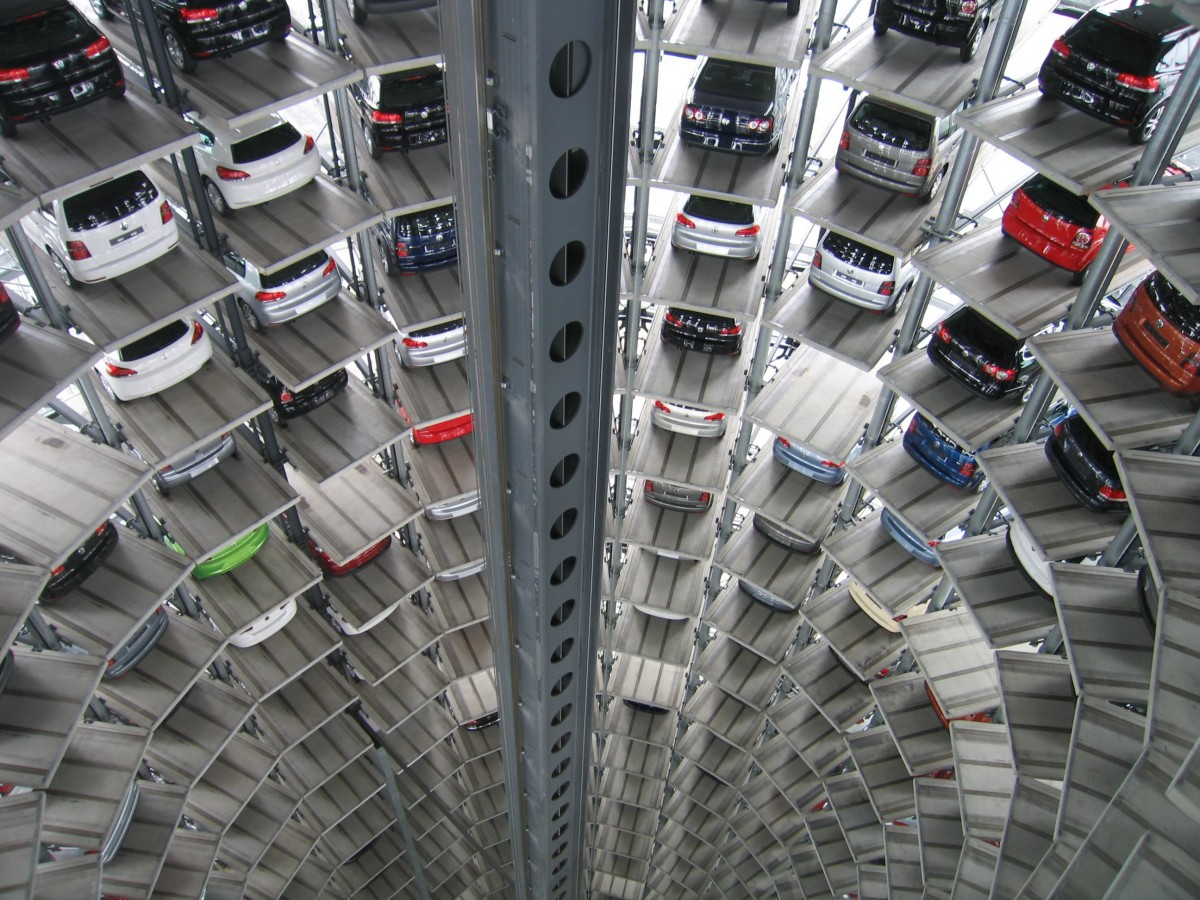
\includegraphics[width=\linewidth]{car-tower}}

% UNIVERSITY-SPECIFIC ADJUSTMENTS
% or: a product line of product-line lectures ;-)
% usage: \def\university{ulm}

\ifdefined\university
\else
\def\university{}
\fi

\newcommand{\ifuniversity}[3][]{\ifthenelse{\equal{\university}{#2}}{#3}{#1}}
\newcommand{\unlessuniversity}[3][]{\ifuniversity[#3]{#2}{#1}}
\newcommand{\inputuniversity}[1]{\IfFileExists{#1-\university}{\input{#1-\university}}{}}

% TITLE
\title{Software Product Lines} % default title for the course
\ifuniversity{ulm}{\title{Software Product Lines}}
\ifuniversity{bern}{\title{Software Product Lines}}
\ifuniversity{magdeburg}{\title{Implementation Techniques for Software Product Lines}}
\ifuniversity{wernigerode}{\title{Requirements Engineering II -- Software Product Lines}}

% LECTURERS AND TUTORS
\makeatletter
\let\author@old\author
\renewcommand{\author}[1]{
	\ifuniversity{ulm}{\author@old{Thomas Thüm, Chico Sundermann}}
	\ifuniversity{bern}{\author@old{Timo Kehrer, Sandra Greiner}}
	\ifuniversity{magdeburg}{\author@old{Gunter Saake, Elias Kuiter}}
	\ifuniversity{wernigerode}{\author@old{Elias Kuiter}}
	\ifuniversity{recording}{\author@old{#1}}
	\ifuniversity{}{\author@old{#1}}
}
\makeatother

% COLOR SCHEME, LOGOS, PICTURES
\ifuniversity{recording}{
	\renewcommand{\deutsch}[1]{} % no German in English recordings
	\mode<beamer>{\renewcommand{\pic}[2][]{\includegraphics[#1]{#2}}} % avoid annoying tool tips during the recording
	\setpicture[550]{jun22-clouds3} % default picture
}{
	\hypersetup{linkcolor=uulm@text, citecolor=red, filecolor=red, runcolor=red, urlcolor=red, colorlinks=true} % emphasizing links, but not when recording
}

\ifuniversity{ulm}{
	% copied from beamerthemeuulm.sty
	\definecolor{black}{HTML}{000000}
	\definecolor{uulmlogoblue}{HTML}{89a2b3}
	\definecolor{uulmblue}{HTML}{7D9AAA}
	\definecolor{uulmaccent}{HTML}{A9A28D}
	\definecolor{green}{HTML}{56AA1C}
	\definecolor{red}{HTML}{A32638}
	\definecolor{orange}{HTML}{DF6D07}
	\definecolor{blue}{HTML}{26547C}
	\ifdarkmode
		\colorlet{green}{green!90!white}
		\colorlet{red}{red!90!white}
		\colorlet{orange}{orange!90!white}
		\colorlet{blue}{blue!90!white}
	\fi

	\uulmlogos{,softvare,,sp,,uulm,}
	\setpicture[550]{jun22-clouds3} % default picture
}

\ifuniversity{bern}{
	% todo
	\uulmlogos{unibe}
}

\ifuniversity{magdeburg}{
	% OVGU colors: https://www.cd.ovgu.de/Logo_+Farbe_+Schrift/Farbe.html
	% FIN colors: https://www.cd.ovgu.de/Fakult%C3%A4ten/Informatik.html
	\definecolor{uulmaccent}{RGB}{77,77,77} % accent gray
	\definecolor{green}{RGB}{5,165,53} % natural sciences
	\definecolor{red}{RGB}{209,63,88} % mathematics
	\definecolor{orange}{RGB}{243,145,0} % humanities
	\definecolor{blue}{RGB}{0,104,180} % computer science
	\setbeamercolor{mypagenumber}{fg=white,bg=blue}
	\setbeamercolor{titlebox}{fg=white,bg=blue}
	\uulmlogos{ovgu-blue}
}

\ifuniversity{wernigerode}{
	\definecolor{uulmaccent}{HTML}{a09377}
	\definecolor{lightaccent}{HTML}{e9e9e5}
	\uulmlogos{hs-harz}
	\setbeamercolor{titlebox}{fg=black,bg=lightaccent}
	\setbeamercolor{mypagenumber}{fg=black,bg=lightaccent}
	\setpicture[400]{wernigerode-castle}
	\renewcommand{\faq}[3]{}
}

% QR CODES
\newcommand{\uploadpractice}{
	\centering
	\ifuniversity{magdeburg}{
		\fancyqr{https://bit.ly/spl-practice}\\[1ex]
		\href{https://bit.ly/spl-practice}{\texttt{bit.ly/spl-practice}}
	}
}